\documentclass{article}

% preamble.tex source: Templates for CCSC Conferences (paper_template)
% https://github.com/ccsc-journal/ccsc-editor/tree/master
\input{preamble}

\addbibresource{paper.bib}

%path to figures - \usepackage{graphicx} is included in preamble.tex
\graphicspath{{figures/}}

\title{Performance Scalability Comparison of Shell Fur and Groom-Based Strand Fur in Unreal Engine\footnote{CSCI 693 Research Methods in Computer Science, Spring 2026}}

\author{
  Luke Sakal\affmark[1], Shelley Wong\affmark[2]\\
  \affmark[1]Computer Science\\
  \affmark[2]Computer Science Department\\
  California State University, Chico\\
  Chico, CA 95929\\
  \email{\{lesakal,swong26\}@csuchico.edu}
}

\begin{document}
\maketitle

\begin{abstract}
Real-time fur rendering requires balancing visual fidelity against limited computational resources. This paper evaluates the scalability of two Unreal Engine fur-rendering approaches: a custom Material-based shell fur implementation and strand fur generated through Unreal Engine's Groom system. Controlled test scenes were created using static furred meshes and Unreal Blueprints. Performance data was then collected from packaged executables using Unreal Engine's CSV Profiler. Experiments varied fur complexity, visible furred object count, and output resolution. Frame time and GPU time were selected as the primary performance metrics.

Results show that both techniques scale approximately linearly as fur complexity increases. Shell fur had lower baseline frame times and GPU times, but its cost increased more quickly as shell count rose. In constrast, strand fur began with a higher baseline cost, but scaled more gradually across the tested curve counts. In the multiple-object test, shell fur maintained lower frame times and GPU times than the Groom-based strand fur. Output resolution had comparatively little effect on either method. These findings suggest that shell fur is well suited for scenes containing several simple static furred objects when shell counts remain moderate, while Groom-based strand fur may be more appropriate for high-detail assets.
\end{abstract}

\section{Introduction}

\subsection{Context and Background}

Rendering realistic fur has been an ongoing challenge in the field of computer graphics. The sheer number of individual hairs on a creature's pelt makes it infeasible to model every strand manually. Additionally, the structure of the hair fiber introduces unique lighting interactions. Rendering methods must consider how to recreate the effect of light on hair. Two broad approaches for rendering hair have become commonplace --- explicit rendering and implicit rendering\cite{andersen2016hybrid}. In explicit rendering, or strand-based rendering, geometry is procedurally created for each strand. This per-strand geometry is then used to inform lighting and motion. In contrast, implicit rendering creates the illusion of fur via volume densities and approximates lighting across.

\subsection{Problem Statement and Research Question}

It is widely accepted that explicit rendering techniques require greater computational resources compared to implicit. However, there is a lack of literature that quantifies the performance and scalability differences between these approaches. For real-time rendering applications, like video games, tradeoffs between performance and visual fidelity are important considerations. Depending on a project's goals and constraints, different techniques may be better suited to it than others. Resource limitations, number of furred objects, the prominence of furry characters, and desired fur appearance can all demand different levels of efficiency and quality.

This paper evaluates the performance and scalability of common real-time fur rendering techniques within Unreal Engine. More specifically, how does the real-time performance of Material-based shell fur and Groom-generated strand fur scale as fur complexity, visible furred-object count, and output resolution increase?

\subsection{Significance of the Study}

Real-time fur rendering must balance visual fidelity against limited resource budgets. This study aims to contribute practical performance data by comparing how shell and strand fur scale as fur complexity, visible furred-object count, and output resolution increase. These results can help inform technique selection for real-time scenes with different performance constraints and visual goals.

\subsection{Scope and Organization}

This paper compares shell fur and strand fur implementations in Unreal Engine through a set of controlled performance tests. The tests vary fur complexity, number of visible furred objects, and output resolution. The study is limited to static meshes, simplified fur assets, a single directional light, and a single hardware configuration. It does not attempt to establish formal visual equivalence between shell and strand counts.

The rest of the paper is organized as follows. Section 2 reviews related work in the domain of fur and hair rendering. Section 3 describes the fur implementations and experiment design. Section 4 presents the results. Section 5 discusses the findings, limitations, and future work. Finally, Section 6 concludes the paper.

\section{Literature Review}

In 1989, Kajiya and Kay introduced a solution for realistic fur rendering\cite{kajiya}. They proposed the use of three-dimensional texture maps, which they called texels, to render fur volumetrically rather than as explicit strands. Alongside this, they introduced an anisotropic lighting model that treated hair and fur fibers as small cylinders, allowing for greater realism in lighting. Lengyel et al. demonstrated a new volumetric fur rendering technique which allowed for real-time rendering over arbitrary topology\cite{lengyel}. Their solution involved creating shells, stacks of the surface mesh extruded along the normals, layered concentrically around the mesh. A semi-transparent, two-dimensional texture for the fur was then applied to these layers, creating the appearance of voluminous fur. To hide visual imperfections left by the shells, Lengyel et al. rendered fins around the silhouette of the mesh. Lengyel et al. adapted the Kajiya-Kay lighting to work with their approach\cite{lengyel}.

The Kajiya-Kay lighting model has served as the base for later hair and fur lighting models. Marschner et al. built off Kajiya-Kay to develop a lighting model which simulates light scattering in human hair fibers\cite{marschner}. While this method captured additional lighting information, such as secondary highlights, the added complexity made it more computationally expensive than the Kajiya-Kay model. A year later, Scheuermann introduced another lighting method based on Kajiya-Kay that approximated the additional lighting captured in the work of Marschner et al\cite{scheuermann}, trading accuracy for lower computational cost. Additional work has been done to improve the realism of the Marschner lighting model and the efficiency of those evolutions\cite{chiang, deon}.

Outside of lighting, fur appearance also needs to account for variation between fur types, such as the difference between the undercoat and guard hairs\cite{andersen2016hybrid}. The density of the undercoat makes rendering explicit geometry generally infeasible\cite{chiang}. In addition to this, the physical structure of an animal's fur can vary between species\cite{chiang}. Anderson et al. found that combining volumetric and strand-based fur provided a solution for this problem. Volumetric fur had a good visual resemblance to the undercoat while the strand-based fur better matched the appearance of guard hairs\cite{andersen2016hybrid}. There are also other tricks to handle the undercoat outside of volumetric rendering. For the strand-based shown in the 2016 animated film \textit{Zootopia}, researchers at Walt Disney Animation Studios faked the undercoat using shading\cite{chiang}. To address species-dependent fur appearance in the film, they varied azimuthal roughness on a per-species basis.

Other research has sought to improve the efficiency of strand-based hair and fur rendering through a variety of techniques. Bhokare et al. presented a method to generate hair strand geometry on-the-fly using the GPU and hair meshes\cite{bhokare}. Their research showed considerable performance improvement, though they note that their approach cannot handle arbitrary hairstyles. Neural nets have also been employed to this end, both to control strand LOD and to generate strand geometry\cite{wei,zhu}.

Existing work largely focuses on improving visual realism or computational efficiency, with greater realism often accompanied with greater expense and vice versa. Comparatively little research provides direct, quantitative data on how the different techniques scale under increasing pressure, which is a common concern in real-time environments. This lack of comparative data limits the ability to determine which techniques are best suited to specific use cases, beyond the general understanding that strand-based methods are more computationally expensive.

\section{Methodology}

\subsection{Implementation Details}
We created shell fur and strand fur using Unreal Engine 5.7.4. The final result of both is showcased in Figure~\ref{fig:monke}. Shell fur was accomplished using a custom Actor Component class and a custom Material. In our initial implementation, the Actor Component class duplicated the base static mesh component and passed relevant parameters to the Material. Initial testing showed that this approach led to a rapidly growing number of draw calls, even when visual quality hit a ceiling.

\begin{figure}[htbp]
    \centering
    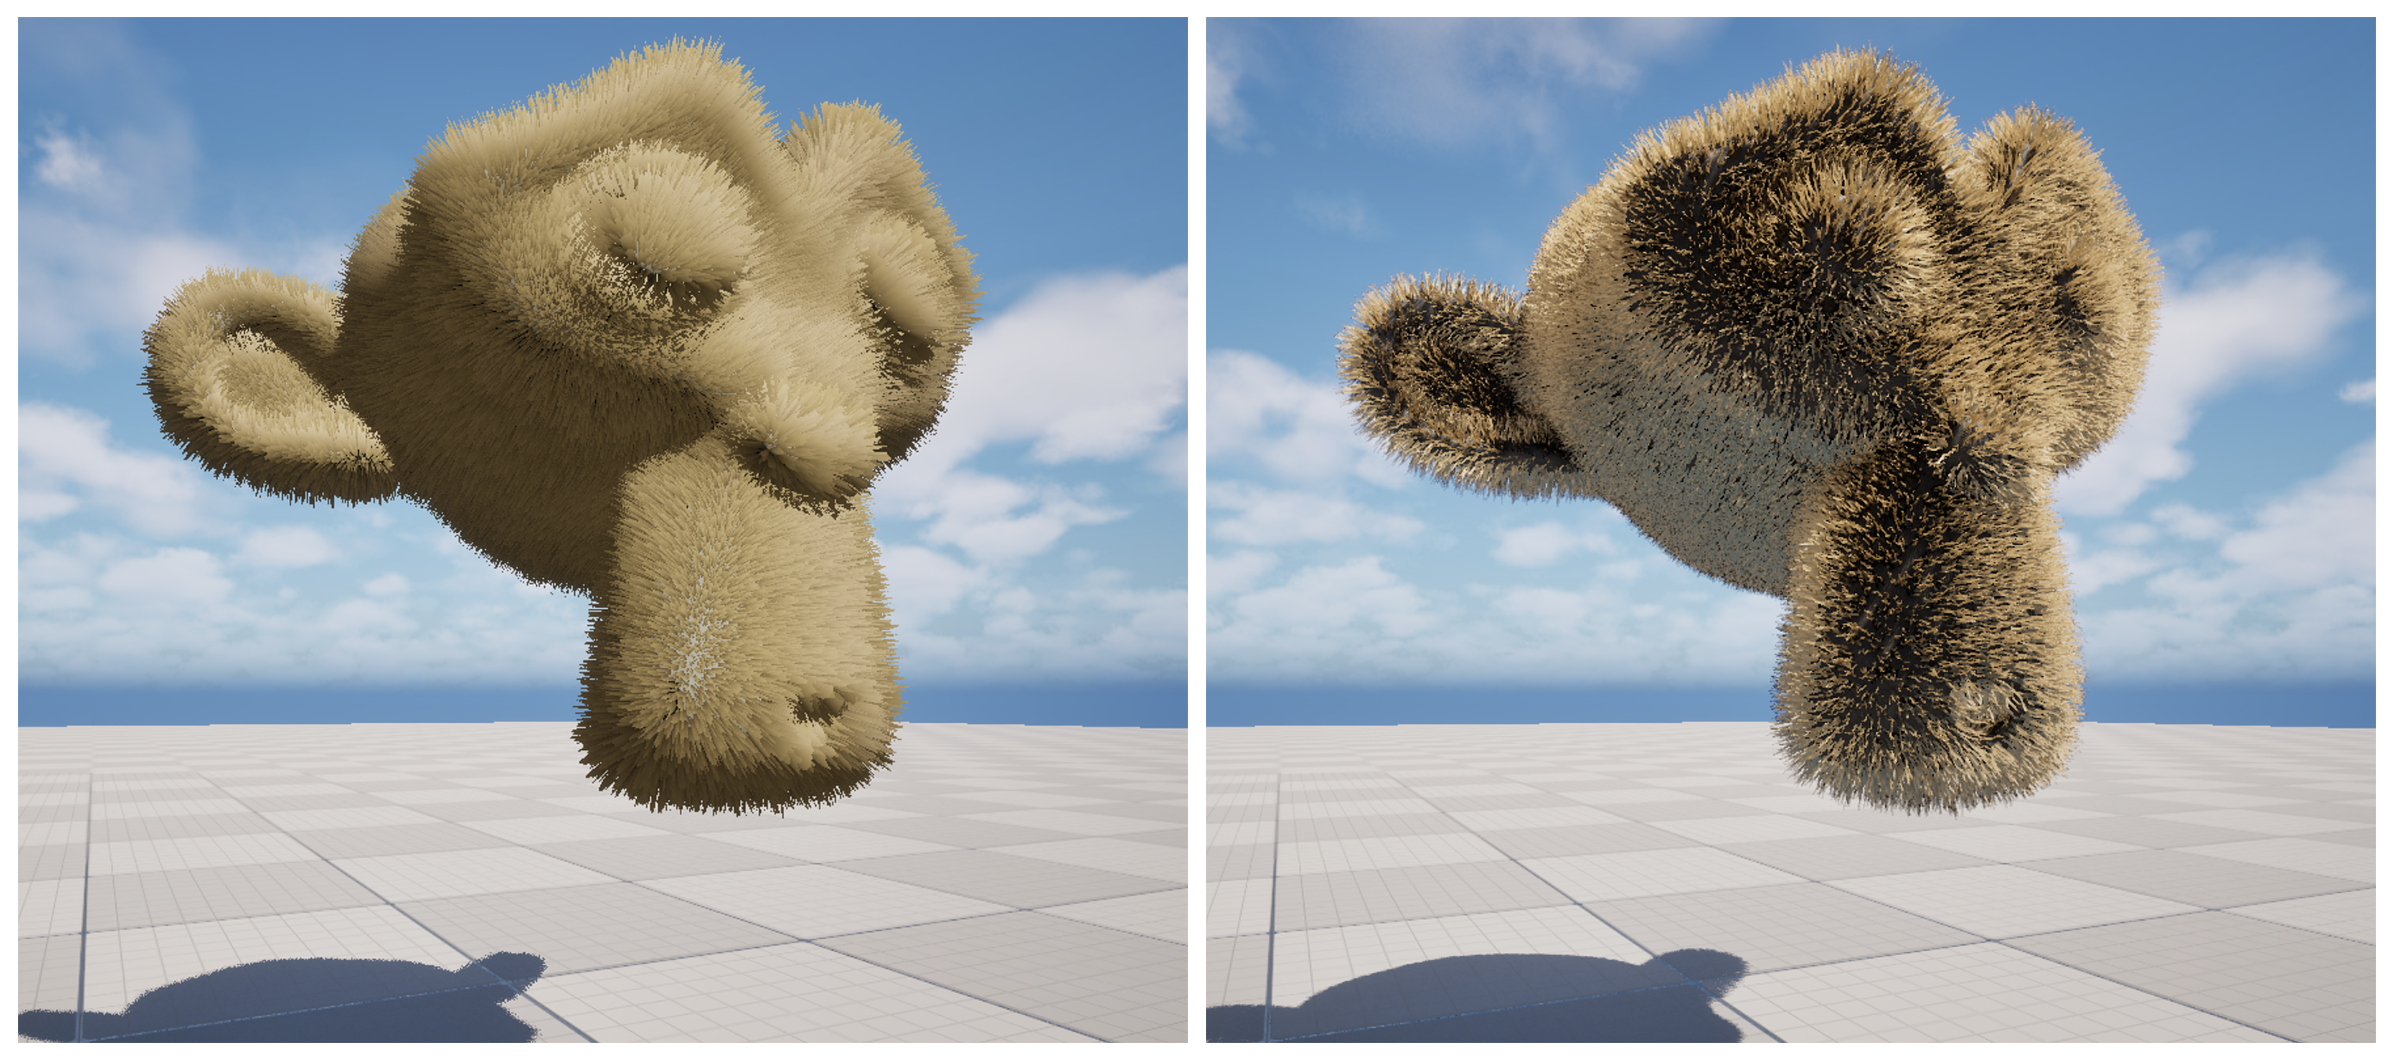
\includegraphics[width=\linewidth]{Figures/Showcase/ExampleMonke.png}
    \caption{Side-by-side images showing a subdivided version of Blender's Suzanne model with shell fur (left) and strand fur (right).}
    \label{fig:monke}
\end{figure}

This led to a second implementation which uses an instanced static mesh component (ISM) instead of duplicating the base static mesh. An ISM contains multiple copies of the assigned static mesh, consolidating collision properties, material properties, and draw calls\cite{EpicGamesISM}. There is no visual difference between the implementations and the ISM version greatly reduced the number of draw calls (see Figure~\ref{fig:base-mean-shell-dc-sr-sub1}). As such, we treat the ISM version as the primary shell fur implementation in this paper.

The Material performs extrusion along the normals using world position offset (WPO), calculates the density of the fur using a noise-based texture, and then applies the modified Kajiya-Kay lighting described by Lengyel et al. with a slight adjustment of our own. The lighting equation used by Lengyel et al. can be written as:

\begin{equation}
\begin{aligned}
\mathrm{HairLighting}(u, v)
&= K_a + K_d \left(1 - u^2\right)^{P_d/2}
  + K_s \left(1 - v^2\right)^{P_s/2}, \\
u &= T \cdot L, \\
v &= T \cdot H.
\end{aligned}
\end{equation}

Our adjustment scales the computed lighting by an additional directional attenuation term, implemented as (NdotL + 0.1). Without this change, the material failed to attenuate lighting in occluded areas. Using the full value of $(N \cdot L)$ created overly harsh shadows. The implementation does not attempt to create accurate cast shadows for the fur. For the exact lighting code, see Listing~\ref{lst:shell-lighting}.

It should be noted that our shell fur Material is custom lit. Rather than going through Unreal's shading pipeline, it uses a custom Material node to calculate the emissive color using the aforementioned lighting equation. While it is possible to use default Unreal Engine lighting instead, we found that it lacked the band-like highlights that the custom lighting provides.

Creation of strand fur was handled via Unreal Engine's Groom system, which uses Groom assets to render hair strands. We created a variety of Groom assets using Blender, an open-source 3D software. The same noise-based texture used for shell fur density was used as a density mask during the creation of the Groom assets. We controlled the number of curves in Blender to create assets with a varying quantity of strands. After importing the asset, we attached it to its corresponding static mesh and applied any transformations necessary to match it to the static mesh.

Unreal Engine handles lighting here, unlike in the shell fur implementation. Unreal's groom lighting system uses a variety of approximation techniques to get a realistic appearance. This includes approaches like dual scattering, which approximates the scattering of light upon hitting a hair fiber, and voxelization --- a method that create a density volume for a groom asset which can be used to inform hair shadowing\cite{EpicGamesGroomWP}. We use Unreal's default hair material without any modifications.

To improve visual quality, we made several tweaks to the default Groom settings. These included increasing strand base width, decreasing strand tip width, and enabling stable rasterization. To lessen shadow noise, we also enabled the Cast Deep Shadows option on the directional light used in the scenes. For fairness, we also enabled this lighting option for shell fur scenes. These settings remained stable across all test cases. 

Even with these options, cast shadows for our strand fur remained very noisy. While it may be possible to minimize this issue by tweaking voxel-related parameters, we found that enabling ray traced shadows for the directional light greatly reduced the noise. See Figure~\ref{fig:rt-shadowing} to view a side-by-side of the shadowing quality with and without ray traced shadows. Since this option changes the shadowing pipeline, we decided to perform a separate set of tests that use this option. This was done for both shell and strand fur. 

\begin{figure}[htbp]
    \centering
    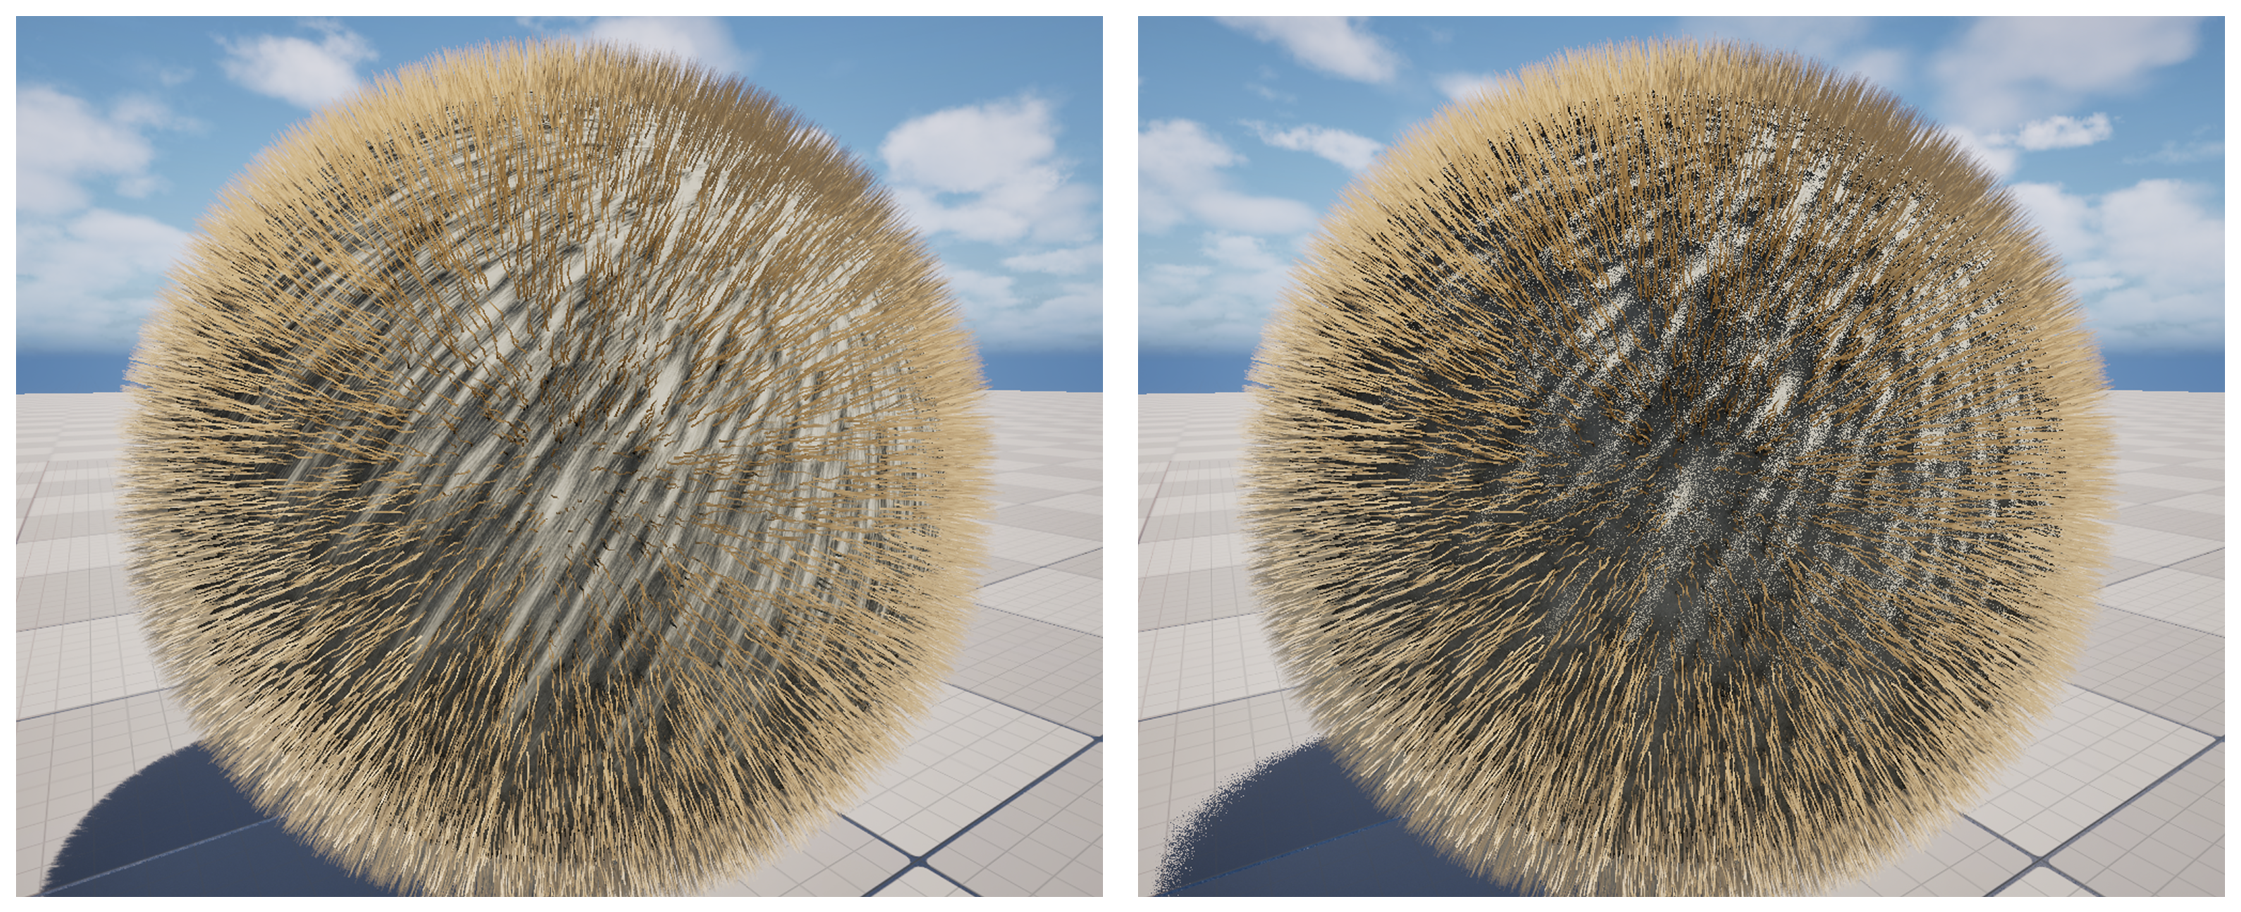
\includegraphics[width=\linewidth]{Figures/Showcase/Sphere_ShadowComparison.png}
    \caption{Sparsely furred sphere with ray traced shadows (left) and without (right).}
    \label{fig:rt-shadowing}
\end{figure}

\subsection{Experiment Design}
We created different levels to set up meshes, lighting, and rendering information. Unreal blueprints define repeatable scene behavior, including camera settings, motion, duration of the run, and the starting or stopping the CSV Profiler. The same level and blueprint were used across multiple runs. 

To avoid overhead from the Unreal Editor, we packed the project into an executable file which would run the level specified prior to packaging. The development build configuration was selected for packaging. The resulting executable was run on a Windows 11 system with an AMD Ryzen 7735HS CPU, 32 gigabytes of RAM, and an Nvidia GeForce RTX 4070 GPU. Unreal's CsvProfiler tool is used to save performance data with its start and stop controlled via blueprints. Prior to starting the profiler, there is fixed warm-up period specified by all the blueprints. During this, resolution and graphics quality are set, vsync is disabled, and frame rate limits are removed. Graphical quality was set to Unreal's "Epic" preset and Material quality was set to high. Unless otherwise noted, resolution was set to 1920x1080.

We tested several different scenes, varying the complexity level of a single variable to determine effects. The base test, which all variations of the shell fur and strand fur implementations went through, consists of a single furred sphere at the center of a rotating camera. The camera distance remains fixed in respect to the sphere to prevent screen space variation. Fur length is also fixed under the same reasoning. Camera rotation was added to capture information for different lighting angles. Table \ref{table:basic-test} shows the different workloads the basic test covers. For each workload, the scene would run ten separate times, recording 60 seconds of performance data.

\begin{table}[ht]
\caption{Base Test Workloads}
\label{table:basic-test} % is used to refer this table in the text
\centering % used for centering table
\begin{tabular}{c c c} % centered columns (4 columns)
\hline\hline %inserts double horizontal lines
Case & Shell Fur (no. of shells) & Strand Fur (no. of curves)\\ [0.5ex]
\hline
1 & 8 & 8,000 \\ % inserting body of the table
2 & 16 & 16,000 \\
3 & 32 & 32,000 \\
4 & 64 & 64,000 \\
5 & 128 & 128,000 \\ 
6 & 256 & 256,000 \\ 
7 & 384 & 384,000 \\ 
8 & 512 & 512,000 \\ 
9 & 768 & 768,000 \\ [1ex] % [1ex] adds vertical space
\hline %inserts single line
\end{tabular}
\end{table}

The next set of tests attempt to measure performance by increasing the number of furry actors in the scene. This was done by setting a varying number of furred spheres in a grid-like pattern. The workload began as a single furred sphere and progressed, two at a time, to a max of nine spheres. To ensure that all spheres were visible, the camera was fixed. Shell count and strand count were also fixed --- specifically at 64 shells and 128,000 curves. We chose these values as they offered visual stability and offered good fur coverage. The scene was set to record 30 seconds of performance data. Five runs were performed for each workload.

Our final testing configuration used the same set up as the basic test --- a single furred sphere at the center of a rotating camera. However, instead of changing the number of shells or strands, we altered video resolution instead. We tested 1280x720, 1600x900, 1920x1080, and 2560x1440. The monitor's native resolution was 2560x1440. Shell and strand counts were fixed similar to the multiple sphere test, with 64 shells and 128,000 curves, respectively.

\subsection{Code Listings}

\begin{lstlisting}[caption=Shell Fur Material Lighting, label={lst:shell-lighting}]
float3 camDir = normalize(camPos - worldPos);

float3 T = normalize(hairDir);   // hair dir at each vertex
float3 L = normalize(-lightDir); // light dir
float3 V = normalize(camDir);    // eye dir

float3 H = normalize(L + V);

float u = dot(T, L);
float v = dot(T, H);

float oneMinusU2 = saturate(1.0 - u * u);
float oneMinusV2 = saturate(1.0 - v * v);

float diffuseTerm = pow(oneMinusU2, diffusePow * 0.5);
float specTerm = pow(oneMinusV2, specPow * 0.5);

float shadowScale = pow(saturate(shellDepth), 1.1);
float selfShadow = lerp(rootDarken, 1.0, shadowScale);

float3 ambientColor = albedo;
float3 diffuseColor = albedo * diffuseStrength;

float NdotL = saturate(dot(T, normalize(lightDir)));

float3 hairLighting =
    ambientColor * selfShadow   +
    diffuseColor * diffuseTerm  * selfShadow +
    specColor    * specStrength * specTerm   * selfShadow;

return hairLighting * (NdotL + 0.1);
\end{lstlisting}

\section{Results}

\subsection{Selected Metrics}

Unreal Engine's CSV Profiler records many performance-related metrics, including frame time, GPU time, draw calls, render thread time, base pass time, and shadow rendering time. Frame time and GPU time are this study's primary metrics as they provide clear, high-level indicators of real-time rendering performance. Frame time captures the total time required to produce each frame and is directly related to the frame rate experienced by the user. GPU time isolates the amount of time spent on rendering work, making it highly relevant for evaluating fur rendering techniques, which engage the GPU during their pipelines.

Other collected metrics are used as supporting diagnostics rather than primary comparison measures. Draw calls and shadow rendering time are useful for identifying implementation-specific behavior and possible bottlenecks.

Throughout the results, “with RT” denotes variants with ray traced shadows enabled for the directional light. This label refers only to the shadowing configuration and should not be interpreted as general ray traced rendering.
Unless otherwise noted, error bars shown in the figures represent 95\% confidence intervals around the mean of runs.

\subsection{Base Test: Scaling with Fur Complexity}

In our base test, increasing fur complexity --- represented by the number of shells or strands --- produces an overall increase in both frame time and GPU time for both shell-based and strand-based rendering techniques.

\begin{figure}[htbp]
    \centering
    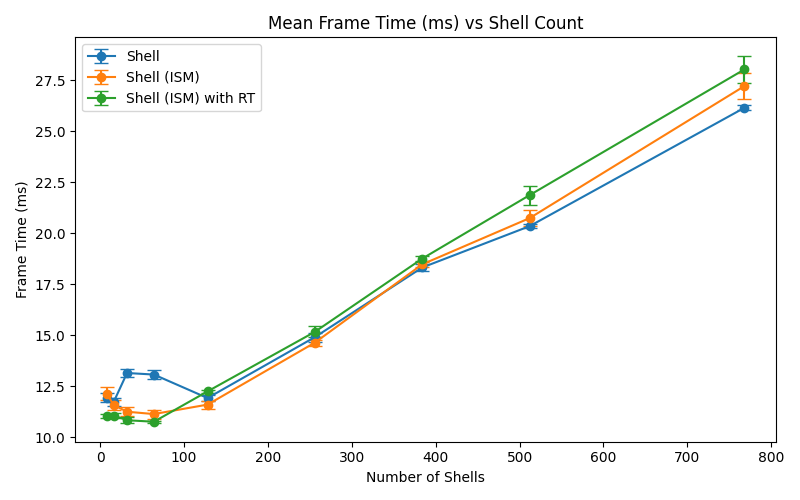
\includegraphics[width=0.8\linewidth]{Figures/BaseTest/Means/Shell/FrameTime_Scaling.png}
    \caption{Line graph showing mean frame time in relation to the number of shells.}
    \label{fig:base-mean-shell-ft}
\end{figure}

\begin{figure}[htbp]
    \centering
    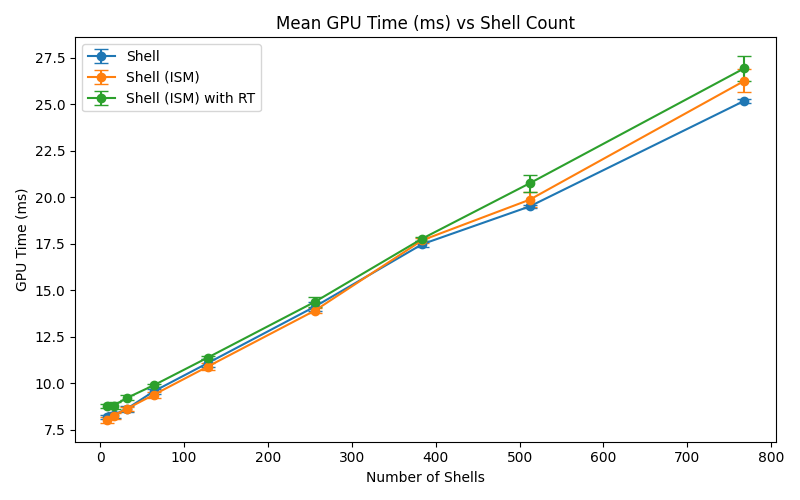
\includegraphics[width=0.8\linewidth]{Figures/BaseTest/Means/Shell/GPUTime_Scaling.png}
    \caption{Line graph showing mean GPU time in relation to the number of shells.}
    \label{fig:base-mean-shell-gpu}
\end{figure}

\subsubsection{Shell-based Fur}

For our shell fur implementations, mean frame times for shell counts under 64 do not follow a clear trend across all variants. Smaller shell counts sometimes have higher frame times than larger shell counts. However, once the shell count exceeds 64, the mean frame time begins to grow in a seemingly linear pattern (Figure~\ref{fig:base-mean-shell-ft}). GPU time growth is more obviously linear, with lower shell counts fitting the trend as well (Figure~\ref{fig:base-mean-shell-gpu}).

The ISM-based shell fur implementation dramatically reduces draw calls and shadow render time, as seen in Figure~\ref{fig:base-mean-shell-dc-sr}. For the non-ISM approach, both these metrics grow linearly in respect to complexity. Comparatively, the ISM variant's draw calls and shadow render time appear constant. In respect to draw calls, there does not appear to be a large difference between tests that use ray traced shadows and those that don't.

\begin{figure}[htbp]
    \centering
    % First subfigure
    \begin{subfigure}{0.475\textwidth}
        \centering
        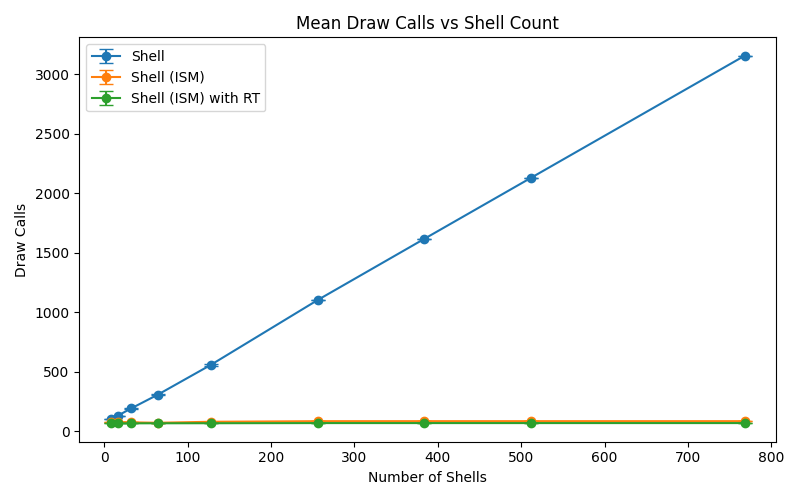
\includegraphics[width=\textwidth]{Figures/BaseTest/Means/Shell/DrawCalls_Scaling.png}
        \caption{Mean number of draw calls.}
        \label{fig:base-mean-shell-dc-sr-sub1}
    \end{subfigure}
    \hfill
    % Second subfigure
    \begin{subfigure}{0.475\textwidth}
        \centering
        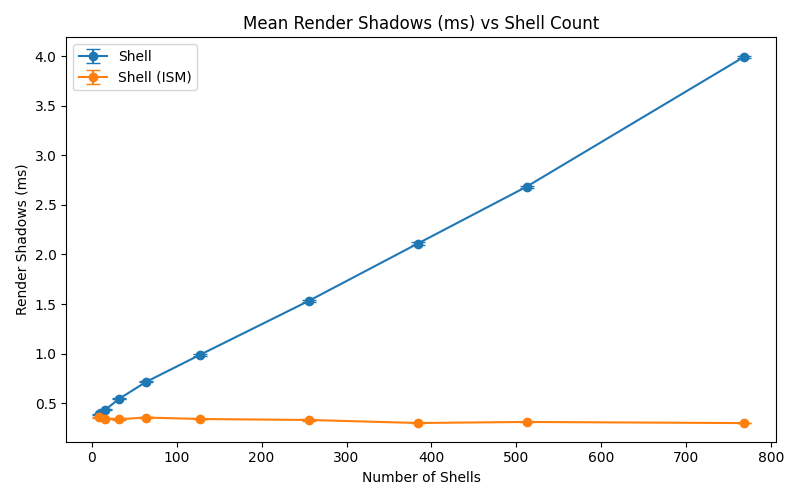
\includegraphics[width=\textwidth]{Figures/BaseTest/Means/Shell/Shadows_Scaling.png}
        \caption{Mean shadow rendering time.}
        \label{fig:base-mean-shell-dc-sr-sub2}
    \end{subfigure}
    
    \caption{Side-by-side line graphs showing the growth of mean draw calls and mean shadow rendering time as shell count increases for ISM-based shell fur and non-ISM shell fur.}
    \label{fig:base-mean-shell-dc-sr}
\end{figure}

\subsubsection{Strand-based Fur}

Figure~\ref{fig:base-mean-strand-ft} and Figure~\ref{fig:base-mean-strand-gpu} show the mean frame time and mean GPU time for strand fur, respectively. Both appear to have close to linear growth across the workloads. Also of note is the tighter time ranges compared to Shell fur. With shell fur, the lowest mean frame time was close to 10 ms while the highest was above 27.5 ms. For strands, the lowest was about 14 ms and the highest was under 24 ms. Similar can be said of the mean GPU time. 

\begin{figure}[htbp]
    \centering
    
\includegraphics[width=0.8\linewidth]{Figures/BaseTest/Means/Strand/FrameTime_Scaling.png}
    \caption{Line graph showing mean frame time in relation to the number of strands.}
    \label{fig:base-mean-strand-ft}
\end{figure}

\begin{figure}[htbp]
    \centering
    
\includegraphics[width=0.8\linewidth]{Figures/BaseTest/Means/Strand/GPUTime_Scaling.png}
    \caption{Line graph showing mean GPU time in relation to the number of strands.}
    \label{fig:base-mean-strand-gpu}
\end{figure}

\begin{figure}[htbp]
    \centering
    
\includegraphics[width=0.8\linewidth]{Figures/BaseTest/Means/Strand/DrawCalls_Scaling.png}
    \caption{Line graph showing number of draw calls in relation to the number of strands.}
    \label{fig:base-mean-strand-dc}
\end{figure}

Draw calls for strand fur remain fairly constant as seen in Figure~\ref{fig:base-mean-strand-dc}. Tests where ray traced shadows were enabled made fewer draw calls than tests without them.

\subsection{Multiple Spheres Test: Scaling with Number of Furred Actors}

Increasing the number of furred spheres visible in the scene correlated with an increase in frame time and GPU time for both shell and strand fur. With strand fur, the jump from a single sphere to three seems to be harsher than with subsequent increases. Compared to strand fur, shell fur frame and GPU time increases at a more gradual pace and is overall faster. It lacks any harsh jumps and nearly forms a straight line (Figure~\ref{fig:spheres-mean-combined}).

\begin{figure}[htbp]
    \centering

    \begin{subfigure}[b]{0.45\linewidth}
        \centering
        
\includegraphics[width=\linewidth]{Figures/MultiSphere/Means/FrameTime_Scaling.png}
        \caption{Mean frame time vs. number of spheres.}
        \label{fig:spheres-mean-ft}
    \end{subfigure}
    \hfill
    \begin{subfigure}[b]{0.45\linewidth}
        \centering
        
\includegraphics[width=\linewidth]{Figures/MultiSphere/Means/GPUTime_Scaling.png}
        \caption{Mean GPU time vs. number of spheres.}
        \label{fig:spheres-mean-gpu}
    \end{subfigure}

    \caption{Performance scaling in the multi-sphere test showing how frame time and GPU time increase with scene complexity.}
    \label{fig:spheres-mean-combined}
\end{figure}

\subsection{Resolution Test: Scaling with Output Resolution}

As exhibited by Figure~\ref{fig:resolution-mean-combined}, increasing resolution did not have much effect on the performance of either fur rendering technique. Strand fur without ray traced shadows exhibits a jump in mean frame and GPU time when going from 1280x720 to 1600x900, but levels out after. The other variants have very little fluctuation across all workloads.

\begin{figure}[htbp]
    \centering

    \begin{subfigure}[b]{0.45\linewidth}
        \centering
        
\includegraphics[width=\linewidth]{Figures/Resolution/FrameTime_Scaling.png}
        \caption{Mean frame time vs. output resolution.}
        \label{fig:resolution-mean-ft}
    \end{subfigure}
    \hfill
    \begin{subfigure}[b]{0.45\linewidth}
        \centering
        
\includegraphics[width=\linewidth]{Figures/Resolution/GPUTime_Scaling.png}
        \caption{Mean GPU time vs. output resolution.}
        \label{fig:resolution-mean-gpu}
    \end{subfigure}

    \caption{Performance scaling with increasing output resolution, showing the impact on frame time and GPU time.}
    \label{fig:resolution-mean-combined}
\end{figure}

\subsection{Key Observations}

Across the tested workloads, frame time and GPU time increased approximately linearly for both methods as fur complexity increased. In the base test, shell fur had lower baseline frame times and GPU times, but its fitted slopes were steeper than those of strand fur, indicating a larger marginal cost as shell count increases. Strand fur began with a higher baseline cost, but its performance increased more gradually across the tested curve counts. In the multiple-sphere test, shell fur maintained lower frame times and GPU times than strand fur. In addition, it scaled more gradually as additional furred actors were added. Output resolution had comparatively little effect on either technique. The ISM-based shell implementation greatly reduced draw calls and shadow render time compared with the non-ISM implementation. However, this did not produce a noticeably large reduction in frame time or GPU time.

\section{Discussion}

\subsection{Interpretation of Results}

The results suggest that the scalability of shell-based and strand-based fur is primarily driven by the amount and detail of fur geometry in a scene. Our base test shows that increasing the number of shells or curves produced a corresponding increase in both frame time and GPU time. For shell fur, GPU time followed a clear linear trend. Frame time was less consistent at low shell counts but became more linear after 64 shells. For strand fur, both frame time and GPU time followed a close-to-linear trend across the tested curve counts. 

The shell fur data also shows that implementation strategy can have a significant effect on certain aspects of scalability. The original non-ISM shell implementation increased draw calls and shadow render time linearly in respect to shell count. The ISM version kept these values nearly constant. This suggests that instancing is hugely influential in improving the efficiency of drawing. That said, frame time and GPU time did not appear to receive a significant boost, which may indicate that the efficiency bottleneck exists elsewhere.

The multiple-sphere test provides a comparison between the two fur rendering techniques at more similar visual qualities than the base test. When fixed at 64 shells and 128,000 curves, shell fur scaled more gradually as the number of furred actors increased, while strand fur showed a larger increase in frame time and GPU time. This suggests that ISM-based shell fur could be a good choice for scenes containing several furred objects, as long as the target appearance can be achieved with a moderate shell count. Strand fur grows more sharply when applied to multiple actors. That said, it also benefits from Unreal Engine's built-in Groom system, including its lighting and shadowing approximations.

The resolution test showed little performance change as output resolution increased from 1280x720 to 2560x1440. This result suggests that neither technique is greatly limited by screen resolution. It also indicates that reducing resolution alone may not substantially improve performance in fur-heavy scenes. More direct controls, such as reducing shell count, curve count, actor count, or shadow quality, are likely to be more effective.

We performed a linear regression using least squares on the results of the base test and the results of the multiple-sphere test. Figure~\ref{fig:base-fits-combined} shows each of the fits for the base tests while Figure~\ref{fig:spheres-fits-combined} shows each of the fits for the multiple-sphere tests. 

\begin{figure}[htbp]
    \centering

    \begin{subfigure}[b]{0.45\linewidth}
        \centering
        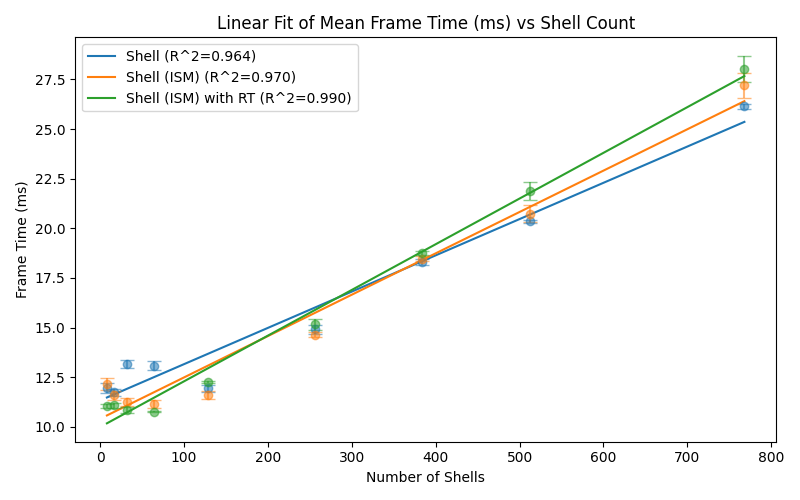
\includegraphics[width=\linewidth]{Figures/BaseTest/Fits/Shell_FrameTime_Fit.png}
        \caption{Shell (ISM): Frame time vs shell count with linear fit.}
        \label{fig:base-fits-shell-ft}
    \end{subfigure}
    \hfill
    \begin{subfigure}[b]{0.45\linewidth}
        \centering
        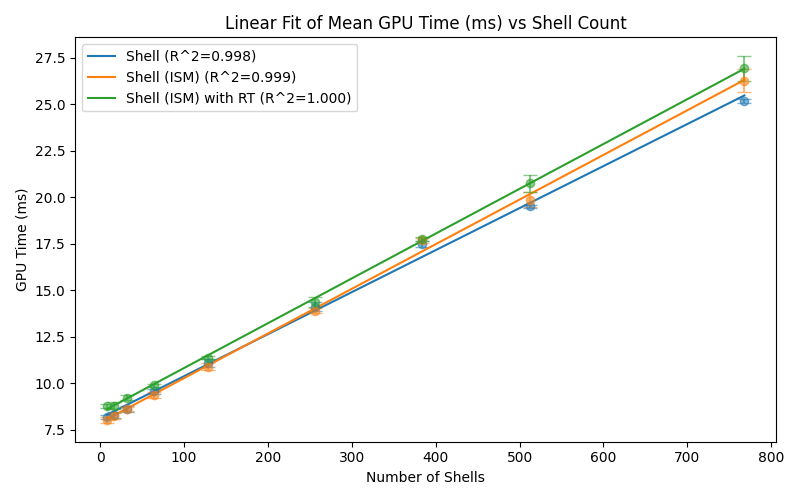
\includegraphics[width=\linewidth]{Figures/BaseTest/Fits/Shell_GPUTime_Fit.png}
        \caption{Shell (ISM): GPU time vs shell count with linear fit.}
        \label{fig:base-fits-shell-gpu}
    \end{subfigure}
    \hfill
    \begin{subfigure}[b]{0.45\linewidth}
        \centering
        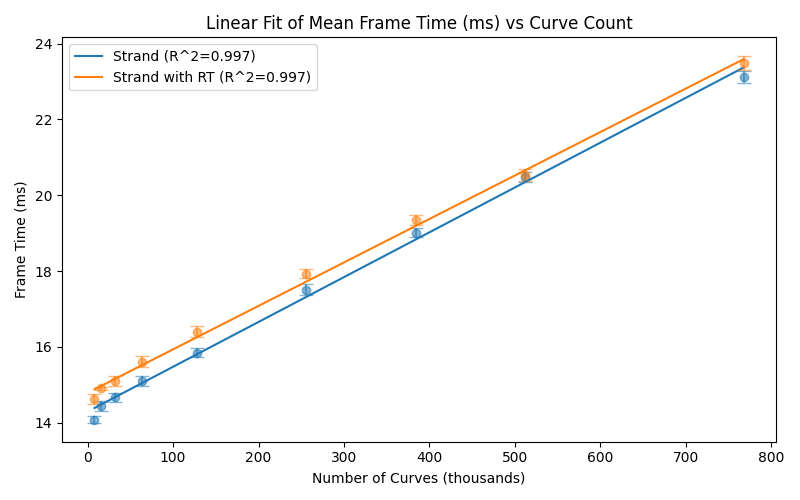
\includegraphics[width=\linewidth]{Figures/BaseTest/Fits/Strand_FrameTime_Fit.png}
        \caption{Strand: Frame time vs curve count with linear fit.}
        \label{fig:base-fits-strand-ft}
    \end{subfigure}
    \begin{subfigure}[b]{0.45\linewidth}
        \centering
        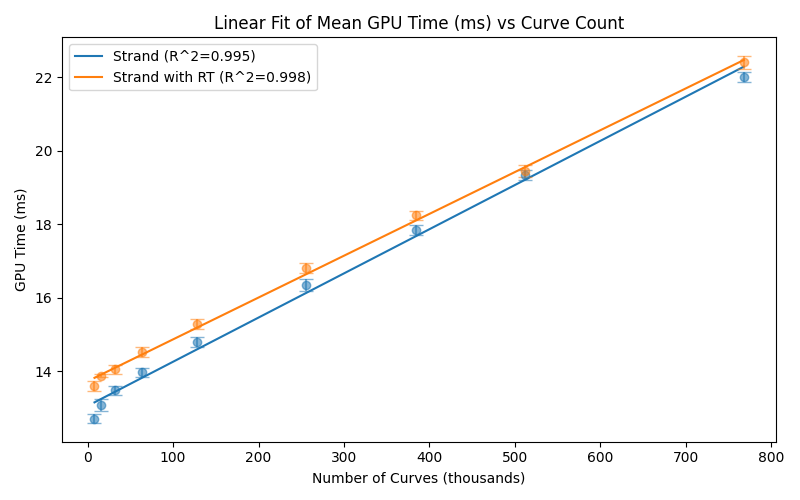
\includegraphics[width=\linewidth]{Figures/BaseTest/Fits/Strand_GPUTime_Fit.png}
        \caption{Strand: GPU time vs curve count with linear fit.}
        \label{fig:base-fits-strand-gpu}
    \end{subfigure}
    \caption{Linear fit results for base test workloads across rendering variants and performance metrics.}
    \label{fig:base-fits-combined}
\end{figure}

\begin{figure}[htbp]
    \centering
    \begin{subfigure}[b]{0.45\linewidth}
        \centering
        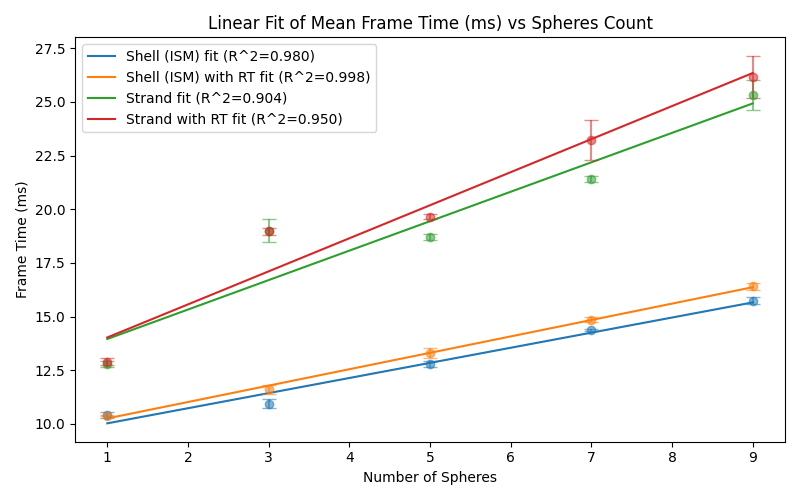
\includegraphics[width=\linewidth]{Figures/MultiSphere/Fits/FrameTime_Fit.png}
        \caption{Frame time vs number of spheres with linear fit.}
        \label{fig:spheres-fits-ft}
    \end{subfigure}
    \hfill
    \begin{subfigure}[b]{0.45\linewidth}
        \centering
        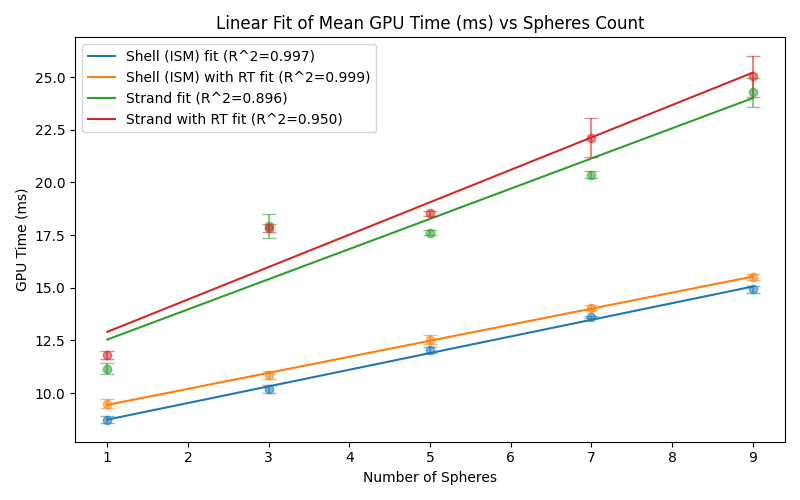
\includegraphics[width=\linewidth]{Figures/MultiSphere/Fits/GPUTime_Fit.png}
        \caption{GPU time vs number of spheres with linear fit.}
        \label{fig:spheres-fits-gpu}
    \end{subfigure}

    \caption{Linear fit results for multi-sphere workload showing performance scaling with increasing scene complexity.}
    \label{fig:spheres-fits-combined}
\end{figure}

By examining the slope of the linear fits calculated for the base test (see Table~\ref{table:base-fit}), we observe that frame time and GPU time for shell fur grow at about double the rate as strand fur. For the multi-sphere test, the slope ratios are reversed and shell fur frame time and GPU time grow at about half the rate as strand fur (see Table~\ref{table:spheres-fit}). 

\begin{table}[htbp]
\caption{Base Test Linear Fit Results}
\label{table:base-fit}
\centering

\begin{subtable}{\linewidth}
\centering
\caption{Frame Time}
\label{table:base-fit-ft}
\begin{tabular}{c c c c c}
\hline\hline
Variant & Slope & Intercept & $R^2$ & Equation \\ [0.5ex]
\hline
Shell (ISM) & 0.021 & 10.404 & 0.970 & $y = 0.021x + 10.404$ \\
Shell (ISM) with RT & 0.023 & 9.989 & 0.990 & $y = 0.023x + 9.989$ \\
Strand & 0.012 & 14.295 & 0.997 & $y = 0.012x + 14.295$ \\
Strand with RT & 0.011 & 14.790 & 0.997 & $y = 0.011x + 14.790$ \\ [1ex]
\hline
\end{tabular}
\end{subtable}

\vspace{1em}

\begin{subtable}{\linewidth}
\centering
\caption{GPU Time}
\label{table:base-fit-gpu}
\begin{tabular}{c c c c c}
\hline\hline
Variant & Slope & Intercept & $R^2$ & Equation \\ [0.5ex]
\hline
Shell (ISM) & 0.024 & 7.873 & 0.999 & $y = 0.024x + 7.873$ \\
Shell (ISM) with RT & 0.024 & 8.407 & 1.000 & $y = 0.024x + 8.407$ \\
Strand & 0.012 & 13.065 & 0.995 & $y = 0.012x + 13.065$ \\
Strand with RT & 0.011 & 13.737 & 0.998 & $y = 0.011x + 13.737$ \\ [1ex]
\hline
\end{tabular}
\end{subtable}
\end{table}

\begin{table}[htbp]
\caption{Multiple-Sphere Test Linear Fit Results}
\label{table:spheres-fit}
\centering

\begin{subtable}{\linewidth}
\centering
\caption{Frame Time}
\label{table:spheres-fit-ft}
\begin{tabular}{c c c c c}
\hline\hline
Variant & Slope & Intercept & $R^2$ & Equation \\ [0.5ex]
\hline
Shell (ISM) & 0.705 & 9.315 & 0.980 & $y = 0.705x + 9.315$ \\
Shell (ISM) with RT & 0.764 & 9.485 & 0.998 & $y = 0.764x + 9.485$ \\
Strand & 1.372 & 12.580 & 0.904 & $y = 1.372x + 12.580$ \\
Strand with RT & 1.541 & 12.483 & 0.950 & $y = 1.541x + 12.483$ \\ [1ex]
\hline
\end{tabular}
\end{subtable}

\vspace{1em}

\begin{subtable}{\linewidth}
\centering
\caption{GPU Time}
\label{table:spheres-fit-gpu}
\begin{tabular}{c c c c c}
\hline\hline
Variant & Slope & Intercept & $R^2$ & Equation \\ [0.5ex]
\hline
Shell (ISM) & 0.789 & 7.953 & 0.997 & $y = 0.789x + 7.953$ \\
Shell (ISM) with RT & 0.846 & 8.105 & 0.999 & $y = 0.846x + 8.105$ \\
Strand & 1.388 & 13.026 & 0.939 & $y = 1.388x + 13.026$ \\
Strand with RT & 1.554 & 13.001 & 0.968 & $y = 1.554x + 13.001$ \\ [1ex]
\hline
\end{tabular}
\end{subtable}
\end{table}

\subsection{Implications}

These findings provide practical guidance for selecting a fur rendering method in Unreal Engine. Shell fur appears better suited for cases where many static or relatively simple furred objects must be rendered at once, as long as approximate lighting is acceptable. This makes it a reasonable choice for background creatures, or in scenarios where performance must be prioritized over visual fidelity. Strand fur was more expensive in the tested multi-actor scenario, but results suggest that it may scale better as fur detail (the number of strands) increases. As such, strand fur may be a good solution for a character or object that requires a high level of detail.

The results also complicate the common assumption that implicit fur is simply cheaper than explicit fur. Shell fur was faster in the actor-count test, but increasing shell count still produced roughly linear increases in frame time and GPU time. While shell fur had a lower baseline cost in the base test, its cost increases more rapidly as shell count rises. Strand fur begins with a higher baseline cost, but its lower slope produces a narrower performance range, making it more competitive at high curve counts. As such, the advantages of shell fur could be offset if shell count becomes excessive.

\subsection{Limitations}

There are multiple limitations in this study. At its core, the comparison is implementation and engine-specific. Our shell fur implementation uses a custom material and custom lighting rather than Unreal Engine's full lighting pipeline, while the strand fur implementation uses Unreal's Groom system. Neither implementation was perfect, with some visual artefacting present in both under certain conditions. Overall, this is a comparison of two practical methods rather than of the underlying algorithms. 

Since our scenes are relatively simple, relying on static meshes, simple Groom assets, a limited lighting setup, and a single hardware configuration, results could easily differ with more complex setups. Animated meshes, skeletal deformation, collision, physics, multiple lights, production-level Groom assets, better optimized shell fur code, or better optimized Groom settings could all have different impacts on fur performance.

Another crucial limitation to note is that tests do not establish visual equivalence between shell count and curve count. Although 64 shells and 128,000 curves were selected because they provided visually stable fur coverage, the study does not attempt to include a formal visual quality metric. Therefore, results should not be interpreted as a one-to-one comparison of efficiency.

\subsection{Suggestions for Future Research}

Creating a shell fur plugin could improve efficiency and support advanced features better than our Material-based implementation. Support for animated meshes, collision, multiple lights, and motion would open the way for comparisons involving the more advanced capabilities of Unreal's Groom system. Unreal's VertexFactory offers more control over vertex data and may be a good avenue to implement complex behaviors. 

The Groom assets we created for this research are simplistic. It's possible that better quality assets could affect the performance. Similarly, tweaking Groom system parameters, changing voxelization options, and other changes could lead to a better optimized render. Testing production-ready Groom assets would provide more practical data.

Hair cards are another common way to render fur and are often used in games. Although it is an implicit method like shell fur, the approach is distinct. Examining the efficiency and scalability of hair cards would provide additional data that could help developers and artists choose which technique best suits their needs.

\section{Conclusion}

This paper evaluated the scalability of Material-based shell fur and strand fur created via Unreal's Groom system using a series of controlled real-time rendering tests. Results indicate that both methods scale in an approximately linear fashion as fur complexity increases. Shell fur showed some irregularity at low shell counts, but its frame time and GPU time became more linear as shell count passed 64. Strand fur followed a more consistent near-linear trend across the tested curve counts.

The results also show that implementation strategy has a significant effect on shell fur scalability. Using instanced static meshes greatly reduced draw calls and shadow render time compared with the original non-ISM implementation. However, this reduction was not reflected in a decrease in frame time or GPU time, suggesting that the main performance cost may fall elsewhere in the rendering pipeline.

In the multiple-sphere test, ISM-based shell fur maintained lower frame times and GPU times than Groom-based strand fur. Shell fur also scaled more gradually as the number of visible furred actors increased. This suggests that shell fur may be more performant for scenes containing several static or relatively simple furred objects, provided that the desired appearance can be met using a moderate shell count. Strand fur was more expensive in this scenario, but it provides a more integrated rendering path through Unreal Engine's Groom system, thus benefiting from more advanced lighting and shadowing.

Output resolution had comparatively little effect on either method across the tested range, suggesting that these scenes were limited more by the amount of fur geometry than by pixel count. Therefore, reducing shell count, curve count, or object count would likely improve performance more than lowering resolution in fur-heavy scenes.

Overall, the results do not show that one fur rendering method is necessarily superior. Instead, they show that shell fur is a scalable approximation when implemented efficiently and used at moderate shell counts. Meanwhile, strand fur offers a generally more expensive approach, but one that may actually handle increasing detail with greater stability. Because this study uses simplified static assets and does not establish formal visual equivalence between shell and strand workloads, the results should be interpreted as a practical comparison of two Unreal Engine implementations rather than a general ranking of implicit and explicit fur rendering methods.

\medskip

\printbibliography

\end{document}
